\documentclass[a4paper,12pt]{article}
%\usepackage{ngerman}
\usepackage{soul}
\usepackage{mathtools}
\usepackage{amssymb,amsmath,amsfonts}
\usepackage{cancel}
\usepackage[utf8]{inputenc}
\usepackage{graphicx}
\usepackage{geometry}
\usepackage[autostyle=true,german=quotes]{csquotes}
\usepackage{gensymb}
\usepackage{units}
\usepackage{fancyhdr}
\usepackage[nottoc,numbib]{tocbibind}
\usepackage{abstract}
\usepackage[font=small,labelfont=bf]{caption}
\usepackage[
%style=alphabetic,
%citestyle=alphabetic,
citestyle=numeric,
sorting=nty
]{biblatex}

\usepackage{hyperref}
\hypersetup{
    colorlinks,
    citecolor=black,
    filecolor=black,
    linkcolor=black,
    urlcolor=black
}

\newcommand{\todo}{\textbf{\textit{TODO}} }

\addbibresource{./../lib/lib.bib}
\addbibresource{../solensim.bib}
\graphicspath{{./../figures/}}

\geometry{a4paper, left=25mm, right=25mm, top=20mm, bottom=20mm}

%\pagestyle{plain}
\pagestyle{fancy}
\fancyhf{}
\fancyhead[L]{solensim documentation}
\fancyhead[R]{\today}
\fancyfoot[C]{\thepage}

\renewcommand{\abstractname}{Summary}

\title{solensim project documentation}


\author{Anton Douginets (anton.douginets@physik.hu-berlin.de)
	\and
	Andrii Yanovets (yanoveta@hu-berlin.de)}

\date{\today}

\begin{document}

\thispagestyle{empty}
\maketitle

\begin{abstract}
  \todo
\end{abstract}

\tableofcontents

\newpage

\section{Introduction}
  \todo


\section{Physical model}
  \todo Few general words

  \paragraph{Solenoid geometry} \todo

  \subsection{Beam parameters}
    A symmetrical, axial beam of known radius and energy distribution is assumed; the interactions of electrons within the beam are neglected.
    \paragraph{Electron energy distribution}
    \todo \cite{AREALRF}

    \paragraph{Beam radius}
    \todo \cite{Disser}

    \paragraph{Electron momentum}
    The formulas involving $p_{z,0}$ call for relativistic momentum \cite[p. 27]{Disser}. The energy-momentum relation is:
    \[
      E^2 = p^2 + m_0^2;
    \]
      With SI factors, this yields
    \begin{equation}
	     p = \frac{1}{c}\sqrt{E^2 - m_0^2c^4}.
      \end{equation}

  \subsection{Field calculation}
    For on-axis electrons, only the on-axis $B_z(x)$ field component is relevant \cite{Disser}. The models used to describe this field are listed below.

    \paragraph{Two-loop approximation}
      \todo

  \subsection{Deriving characteristic values}
    \todo

  \subsection{Aberrations}
    \todo
    \paragraph{Spherical aberrations} \todo
      \begin{figure}[h]
        \centering
        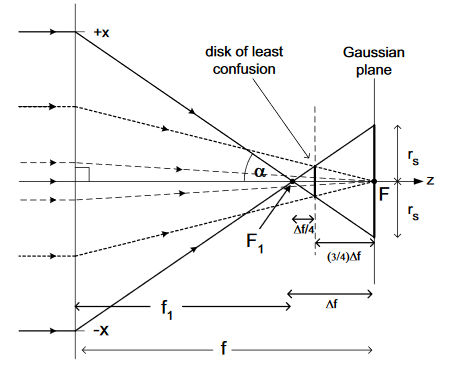
\includegraphics[width=0.75\textwidth]{cs_illustration}
        \caption{Focus shift due to spherical aberrations}
      \end{figure}

      \[
        1/f=const.\cdotp F2
      \]

      \[
        \triangle f\simeq c\cdotp x^{2}
      \]

      \[
        x=f_{1}tan\left(\alpha\right)\simeq f\cdotp tan\left(\alpha\right)
      \]

      \[
        r_{s}=\triangle f\cdotp tan\left(\alpha\right)\simeq\triangle f\cdotp\alpha\approx\left(c\left(f\cdotp tan\left(\alpha\right)\right)^{2}\right)\cdotp tan\left(\alpha\right)=C_{s}tan\left(\alpha\right)^{3}=C_{s}\cdotp\left(\frac{max\left\{ x\right\} }{f-\triangle f}\right)^{3}
      \]

      \[
        \underset{f\approx f_{1}}{=}C_{s}\cdotp\left(\frac{max\left\{ x\right\} }{f}\right)^{3}\quad(1)
      \]

      If $f\cancel{\approx}f_{1}$then replace $f$ in (1) with $f-max\left\{ x\right\} ^{2}\cdotp\frac{C_{s}}{f^{2}}$

  \subsubsection{Chromatic aberrations}
    \todo

\newpage

\section{Project concept and implementation}
  \todo

\newpage

\section{Software manual}
  \todo

\newpage

\printbibliography[
heading=bibintoc,
title={References}
]

%\section{Appendix}
%Also as begin/end environment
%\listoffigures

%\listoftables

\end{document}
